\documentclass[aspectratio=169]{beamer}

\usepackage{pgf}  
\usepackage{tikz}
\usetikzlibrary{arrows}
\usepgflibrary{shapes.arrows} 
\usetikzlibrary{intersections}
\usetikzlibrary{calc}
\usetikzlibrary{fit}
\usetikzlibrary{automata,positioning}
\usepackage{pgfplots,stackengine}
\usepackage{fontspec}
\usepackage{fancyvrb}
\usepackage{wasysym}
\usepackage{unicode-math}
\usepackage{import}
\usepackage{rotating}
\usepackage{gensymb}
\usepackage{chemfig}
\usepackage{rotating}
\usepackage{booktabs}
\usepackage{array}
\usepackage{blkarray}
\usepackage{pifont}
\usepackage{letltxmacro}
\usepackage{wrapfig}
\usepackage{mathtools}
\usepackage{graphbox}
\usepackage{epigraph}
\usepackage{listings}
\usepackage{verbatim}
\usepackage{hologo}
\usepackage{multimedia}
\usepackage{mol2chemfig}
\usepackage{nicematrix}
\usepackage[absolute,overlay]{textpos}
\usepackage[euler-digits,euler-hat-accent]{eulervm}
%\logo{\pgfputat{\pgfxy(.45,.5)}{\pgfbox[center]{\includegraphics[width=1.7cm]{Figures/Bioclipse.png}}}}

\usetheme{Copenhagen}
\usecolortheme{beaver}

\definecolor{uured}{RGB}{153,0,0}
\definecolor{darkpastelgreen}{rgb}{0.01, 0.75, 0.24}

\setbeamercolor{block title}{use=structure,fg=white,bg=uured}
\setbeamercolor*{item}{fg=uured}

\newcommand{\unilogo}{
  \setlength{\TPHorizModule}{1pt}
  \setlength{\TPVertModule}{1pt}
  \begin{textblock}{1}(26,-10)
   
\includegraphics[height=70pt, align=c]{Figures/uu_shadow.png}
  \end{textblock}
  } 

\pgfmathdeclarefunction{gauss}{2}{%
  \pgfmathparse{1/(#2*sqrt(2*pi))*exp(-((x-#1)^2)/(2*#2^2))}%
}
  
\makeatletter
    \newcases{mycases}{\quad}{%
        \hfil$\m@th\displaystyle{##}$}{$\m@th\displaystyle{##}$\hfil}{\lbrace}{.}
\makeatother

\addtobeamertemplate{frametitle}{}{%
    \unilogo
}

\LetLtxMacro{\oldBlock}{\block}
\LetLtxMacro{\endoldBlock}{\endblock}
\renewcommand{\block}{\begin{center}\begin{minipage}{0.8\textwidth}\oldBlock}
\renewcommand{\endblock}{\endoldBlock\end{minipage}\end{center}}
\setlength{\fboxsep}{0pt}

\makeatletter
\newcommand{\srcsize}{\@setfontsize{\srcsize}{4pt}{4pt}}
\makeatother

\begin{document}
\graphicspath{{Figures/}}
\setsansfont[ItalicFont = Optima Italic,
             BoldFont = Optima Bold,
             Ligatures=TeX ]
            {Optima Regular}
\setmainfont[ItalicFont = Optima Italic,
             BoldFont = Optima Bold,
             Ligatures=TeX]
            {Optima Regular}
%\newfontfamily\comment[]{Chalkboard}
\newfontfamily\zA[Ligatures={Common, Rare}, Variant=1] {Zapfino}
\newfontfamily\zB[Ligatures={Common, Rare}, Variant=2] {Zapfino}
\newfontfamily\zC[Ligatures={Common, Rare}, Variant=3] {Zapfino}
\newfontfamily\zD[Ligatures={Common, Rare}, Variant=4] {Zapfino}
\newfontfamily\zE[Ligatures={Common, Rare}, Variant=5] {Zapfino}
\newfontfamily\zF[Ligatures={Common, Rare}, Variant=6] {Zapfino}
\newfontfamily\zG[Ligatures={Common, Rare}, Variant=7] {Zapfino}
\renewcommand\UrlFont{\color{blue}}
\renewcommand\thefootnote{\textcolor{uured}{\arabic{footnote}}}
\setbeamercolor{alerted text}{fg=uured}
\lstset{basicstyle=\ttfamily\scriptsize, frame=single }
\newcommand{\TikZ}{{\lmr Ti\textit{k}Z}}


\title{Ligand-based modeling}   
\author{Jonathan Alvarsson} 
\titlegraphic{
\includegraphics[height=18pt]{Figures/pharmbio-logo-new.png}}
\date{\today} 

\setbeamertemplate{background}{%
    \parbox[c][\paperheight]{\paperwidth}{%
        \vfill
        \hfill
        
\includegraphics[height=0.65\textheight]{Figures/sigill.png}
    }   
}
\begin{frame}[plain]
\unilogo \vspace{1cm} \titlepage
\begin{tikzpicture}[remember picture,overlay]
\tikz[remember picture, overlay] \fill[uured] (current page.north west) rectangle ++(\paperwidth,-0.5cm);
\end{tikzpicture}%
\end{frame}

\setbeamertemplate{background}{}
\renewcommand{\unilogo}{
  \setlength{\TPHorizModule}{1pt}
  \setlength{\TPVertModule}{1pt}
  \begin{textblock}{1}(0,0)
   
\includegraphics[height=27pt, align=c]{Figures/uu.png}
\includegraphics[height=10pt, align=c]{Figures/pharmbio-logo-new.png}
  \end{textblock}
  }

    %\begin{frame}
    %\frametitle{Outline}
    %\begin{minipage}{0.25\textwidth}
    %\mbox{}
    %\end{minipage}
    %\begin{minipage}{0.6\textwidth}
    %\tableofcontents
    %\end{minipage}
    %\end{frame}
    
    \begin{frame}
        \frametitle{Ligand-based modelling}
        \framesubtitle{No target and no structure}

        \begin{block}{Ligand-based modelling}
            \begin{itemize}
                \item In ligand-based modelling we are working without a known target
                \item A series of ligands have a certain effect
            \end{itemize}
        \end{block}
    \end{frame}
    
    \begin{frame}
        \frametitle{Ligand-based modelling}
        \framesubtitle{Similarity principle}

        \begin{block}{Similarity principle}
            \begin{itemize}
                \item Similar substances should behave in a similar fashion
                \item What can we learn by just studying the ligands?
            \end{itemize}
        \end{block}
    \end{frame}

\section{QSAR}

    \begin{frame}
        \frametitle{QSAR}
        \framesubtitle{Quantitative structure–activity relationship}

        \begin{block}{Quantitative structure–activity relationship}
            In QSAR we mathematically describe molecular structure and by machine learning predict molecular properties
            \uncover<2>{
            \begin{itemize}
                \item \alert{QSAR} -- Quantitative Structure-Activity Relationship
                \item \alert{QSPR} -- Quantitative Structure-Property Relationship
            \end{itemize}
            }
        \end{block}
    \end{frame}
    
    \begin{frame}
        \frametitle{QSAR}
        \framesubtitle{Quantitative structure–activity relationship}

        \begin{block}{Quantitative structure–activity relationship}
            QSAR can be used for predicting almost any molecular properties:
            \begin{itemize}
                \item Biological activity
                \item Risk management, toxicology
                \item \ldots
            \end{itemize}
        \end{block}

    \end{frame}


    \begin{frame}
        \frametitle{QSAR}
        \framesubtitle{Quantitative structure–activity relationship}
        \centering

        \begin{tikzpicture}
                \node (structures) [text width=2.4cm, rectangle, text centered]
                                  {Molecular structures};
                \node (activity) [text width=3cm, rectangle, 
                                text centered, right of=structures, node distance=3.5cm]
                                {Activity or Property};
                \only<1>{\draw [->] (structures) to (activity);}
                \uncover<2->{\draw [dashed,->] (structures) to (activity);}
            \uncover<2->{
                \node (descriptors) [text width=2.4cm,rectangle, node distance=1.5cm,
                                     text centered, below of=structures]
                                    {Molecular descriptors};
                \draw [->] (structures) to (descriptors);
            }
            \uncover<3->{
                \node (model) [text width=3cm,rectangle, node distance=1.5cm,
                                     text centered, below of=activity]
                                    {Mathematical model};
                \draw [->] (descriptors) to (model);
            }
            \uncover<4->{
                \draw [->] (model) to (activity);
            }
            \uncover<5->{
                \footnotesize
                \node (combine) [text width=3.5cm,rectangle, node distance=2.2cm,
                                     text centered, below left of=descriptors]
                                {\color{darkpastelgreen}Good to combine many different descriptors};
                \draw [->, darkpastelgreen] (combine) to (descriptors);
                \node (validation) [text width=5.6cm,rectangle, node distance=2.2cm,
                                     text centered, below right of=model]
                                {\color{darkpastelgreen}Machine learning};
                \draw [->, darkpastelgreen] (validation) to (model);
                \node (more) [text width=4cm,rectangle, node distance=2cm,
                                     text centered, above left of=structures]
                                {\color{darkpastelgreen}More structures often lead to better models};
                \draw [->, darkpastelgreen] (more) to (structures);
            }
        \end{tikzpicture}
    \end{frame}

    \begin{frame}
        \frametitle{QSAR}
        \framesubtitle{Quantitative structure–activity relationship}
        \begin{block}{History of QSAR}
            More than 100 years ago it was discovered that the narcotic
            properties of anaesthetizing gases correlated with the their
            solubility in olive oil. 
            \vspace{0.5\baselineskip}

            \alert{The first proper QSAR model was developed in 1962} it
            modeled phenoxyacetic acids regulations of plant growth as a
            function of the compounds lipohilicity. 
        \end{block}
    \end{frame}

\section{Molecular Descriptors}
    \begin{frame}
        \frametitle{Molecular Descriptors}
                \begin{block}{Molecular descriptors} 
A molecular \alert{descriptor} is a \alert{mathematical representation} of a
molecule, often resulting from the \alert{transformation} of the \alert{symbolic
representation} of a molecule into \alert{numbers}
        \end{block}
    \uncover<2->{
    \begin{block}{Simple examples}
    \quad
    \begin{minipage}[c]{0.3\linewidth}
        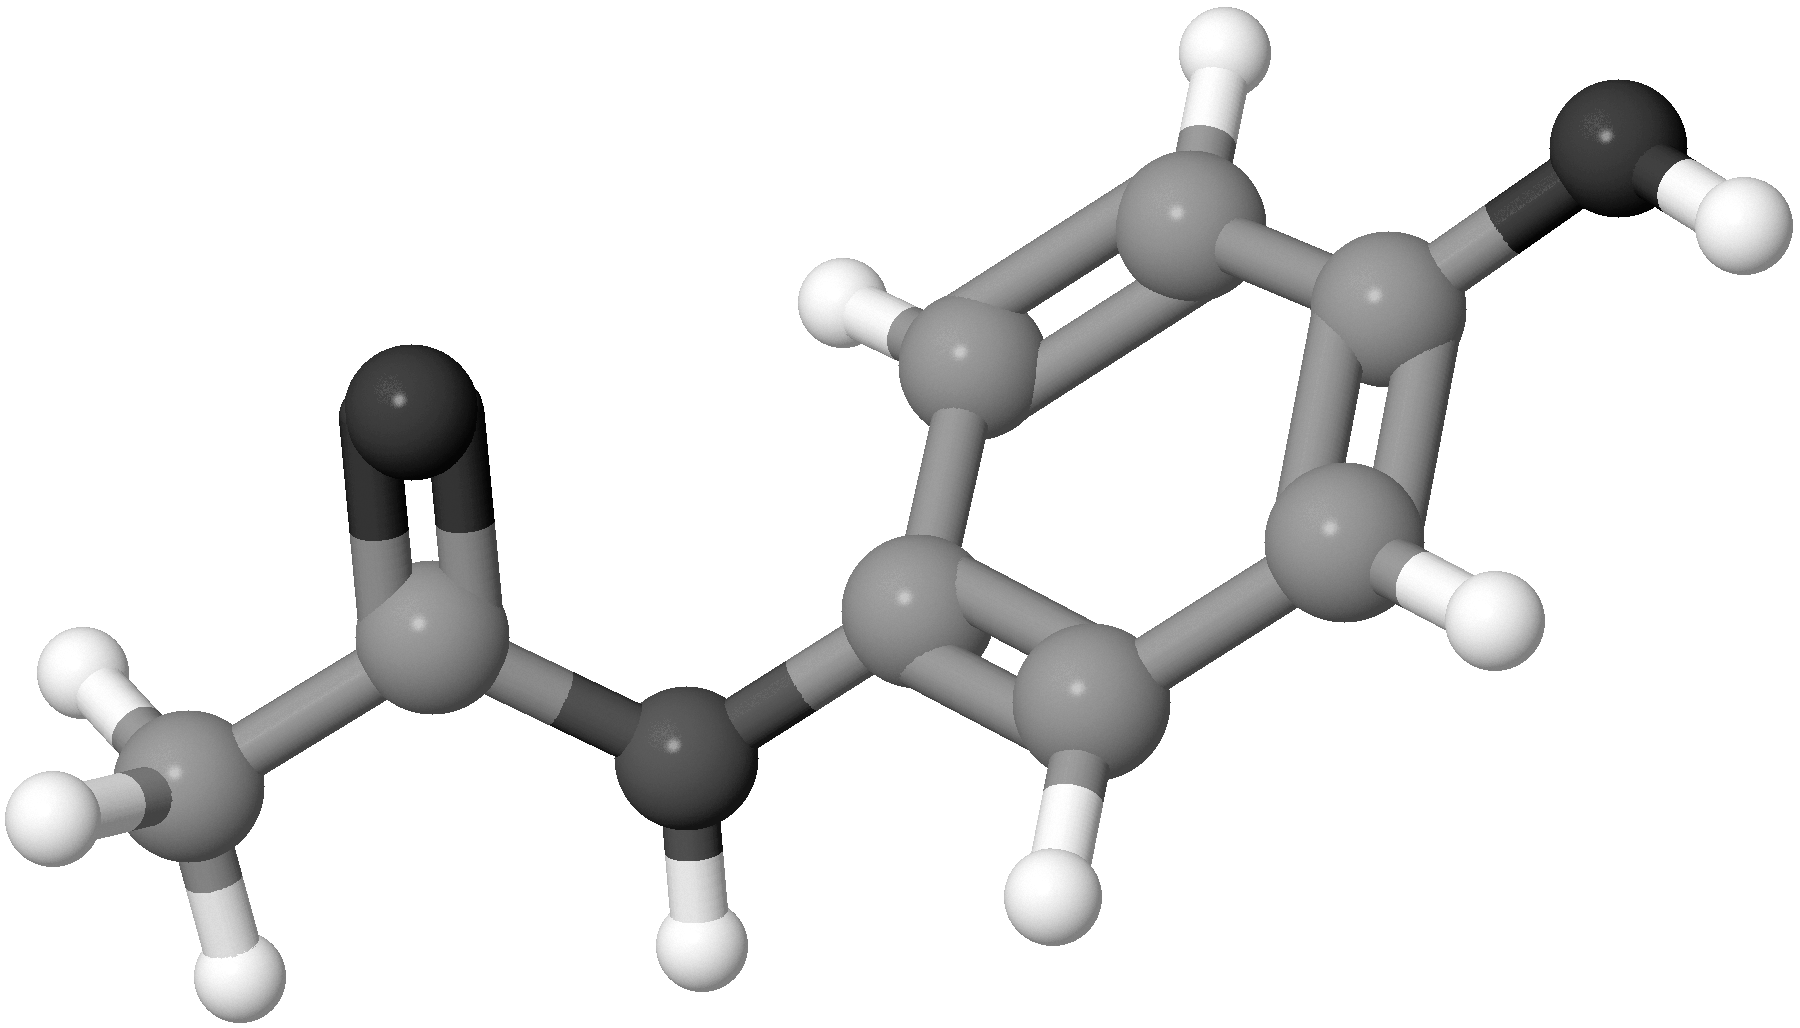
\includegraphics[width=1\textwidth]{figures/paracetamol.png}
    \end{minipage}
    \qquad
    \begin{minipage}[c]{0.4\linewidth}
    \small
    \begin{tabular}{lr}
    \toprule
    Descriptor & Value \\
    \midrule
    Molecular weight          & 151.06 \\
    Number of carbon atoms    & 8      \\
    \bottomrule
    \end{tabular}
    \end{minipage}
    \end{block}}

    \end{frame}

\subsection{Classifications}
       \begin{frame}
        \frametitle{Molecular Descriptors}
        \framesubtitle{Classifications}
        \begin{minipage}[c]{0.6\textwidth}
        \oldBlock{By ``dimensionality''}
        \begin{itemize}
            \item 0D -- molecular weight, number of atoms
            \item 1D -- fragment counts, fingerprints
            \item 2D -- topological descriptors
            \item 3D -- geometrical descriptors
        \end{itemize}
        \endoldBlock
        \end{minipage}
        \hfill
        \begin{minipage}[c]{0.35\textwidth}
        \oldBlock{By data type}
        \begin{itemize}
            \item Boolean
            \item Integer
            \item Real number
            \item Vector
        \end{itemize} 
        \endoldBlock
        \end{minipage}

    \end{frame}

    \begin{frame}
        \frametitle{Molecular Descriptors}
        \framesubtitle{Classifications of descriptors}
        \small
        \begin{block}{Other classification schemas include, \textit{e.g.}, the following classes:}
            \begin{itemize}
                \item Constitutional -- does not take molecular geometry into account
                \item Topological -- based on molecular graphs
                \item Geometrical -- based on 3D structure
                \item Electronic -- based on electronic structure
                \item Physiochemical -- based on lab measurable properties
            \end{itemize}
        \end{block}
        \centering
        \uncover<2->{\color{darkpastelgreen}Classes overlap and descriptors belong to more than one class}
    \end{frame}

\subsection{Examples}

    \begin{frame}
        \frametitle{Molecular descriptors}
        \framesubtitle{Examples}
                \hfill
        \begin{minipage}[c]{0.7\textwidth}
        \oldBlock{Log P}
        \alert{Log P} is a real number physiochemical descriptor. Log P is the
        logarithm of the \alert{partition coefficient}; the the \alert{ratio of
        concentrations} of the studied substance between \alert{water} and
        \alert{octanol}. This affects how easily a drug can reach its intended
        target in the body.
        \endoldBlock
        \end{minipage}
        \hfill
        \begin{minipage}[c]{0.2\textwidth}
        \fbox{\includegraphics[width=1\textwidth]{Figures/funnel.png}}~\rotatebox{90}{\tiny Photo: \texttt{PRHaney}}
        \end{minipage}
        \hfill
    \end{frame}

    \newcommand\tm[2][]{\tikz[overlay,remember picture,baseline=(#1.base),inner sep=0pt]\node(#1){$#2$};}

    \begin{frame}
        \frametitle{Molecular descriptors}
        \framesubtitle{Examples}
        \begin{block}{Wiener index}
        The \alert{Wiener index} $W$ is defined as: the \alert{sum of the lengths} of the
        \alert{shortest paths between} all \alert{pairs of vertices} in the
        chemical graph of the molecule \alert{excluding hydrogens}. It can be
        calculated by \alert{summing the upper right triangle} of the
        \alert{distance matrix} $D$ for the compound:
        \small
        \begin{equation*}
            D\left( \raisebox{-2ex}{\chemfig{ C_a-C_b-[:50,,,1]O_cH }}\right)  = \begin{blockarray}{cccc}
        & \chemfig{C_a} & \chemfig{C_b} &  \chemfig{O_c} \\
            \begin{block}{c(ccc)}
        \chemfig{C_a} &  0 & \tm[a]{1} & \tm[b]{2} \\
        \chemfig{C_b} &  1 & 0 & \tm[c]{1}         \\
        \chemfig{O_c} &  2 & 1 & 0 \\
        \end{block}
        \end{blockarray},\qquad
        W = 1 + 2 + 1 = 4
        \end{equation*}
        \begin{tikzpicture}[overlay, remember picture]
        \node(x)[fit=(a) (b),inner sep=2pt]{};
        \node(y)[fit=(b) (c),inner sep=2pt]{};
        \fill[rounded corners,opacity=.3,fill=uured](x.north west)--(x.south west)--(y.south west)--(y.south east)--(x.north east)--cycle;
        \end{tikzpicture}
        \vspace{-1\baselineskip}
            \end{block}
    \end{frame}

    \begin{frame}
        \frametitle{Molecular descriptors}
        \framesubtitle{Examples}
        \begin{block}{Signature descriptor}
        The \alert{signature descriptor} is a \alert{topological} descriptor using atom type
        information and represented as a list of strings. It is constructed by describing
        the \alert{environment around each atom} in a molecule by describing each atoms
        \alert{neighbouring atoms} out to a specific distance (refered to as
        height). Hydrogens are often skipped.
        \end{block}
    \end{frame}

    \begin{frame}
        \frametitle{Molecular descriptors}
        \framesubtitle{Examples}

        \oldBlock{Atom Signature descriptor for \chemfig{N_a}}
            \hfill
            \begin{minipage}[c]{0.2\textwidth}
            \chemfig{
                    O_fH% 6
           -[:90,,1]C_d% 1
              -[:36]C_e% 2
            =^[:108]N_a% 3
             -[:180]C_b% 4
    =^[:252.1,0.995]N_c% 5
                       (
         -[:323.7,0.7]% -> 1
                       )
} 
            \end{minipage}
            \hfill
            \begin{minipage}{0.7\textwidth}
\begin{tikzpicture}[level distance=1cm,
  level 1/.style={sibling distance=2cm},
  level 2/.style={sibling distance=1cm},
  level 3/.style={sibling distance=1cm}]
  \node(a) {\chemfig{N_a}}
    child {node {\chemfig{C_b}}
      child {node {\chemfig{N_c}}
        child {node {\chemfig{C_d}}}
        }
    }
    child {node {\chemfig{C_e}}
        child {node {\chemfig{C_d}}
            child {node {\chemfig{N_c}}}
            child {node {\chemfig{O_f}}}
        }
    };
    \node(h1)[right of=a, node distance=4cm]{h=0 [N]};
    \node(h2)[below=of h1.west, anchor=west, node distance=1cm]{h=1 [N]([C],[C])};
    \node(h3)[below=of h2.west, anchor=west, node distance=1cm]{h=2 [N]([C]([N]),[C]([C]))};
\end{tikzpicture}
            \end{minipage}
            \hfill
        \endoldBlock
    \end{frame}



    \begin{frame}
        \frametitle{Molecular descriptors}
        \framesubtitle{Examples}
        \oldBlock{Atom signature descriptors for ethanol}
            \hfill
            \begin{minipage}[c]{0.2\textwidth}
            \chemfig{ C_a-C_b-[:50,,,1]O_cH } 
            \end{minipage}
            \hfill
            \begin{minipage}{0.7\textwidth}
            \begin{tabular}{cccc}
            \toprule
            Height & \chemfig{C_a} & \chemfig{C_b} & \chemfig{O_c} \\
            \midrule
            0      & [C] & [C] & [O] \\ 
            1      & [C]([C]) & [C]([C][O]) & [O]([C]) \\
            2      & [C]([C]([O])) & [C]([C][O]) & [O]([C]([C])) \\
            \bottomrule
            \end{tabular}
            \end{minipage}
            \hfill
            \vspace{1\baselineskip}

            Notice that ethanol is so small that signature heights beyond
            height 2 does not add any more information.
        \endoldBlock
    \end{frame}






\subsection{Molecular Fingerprints}

    \begin{frame}
        \frametitle{Molecular Fingerprints}
        \begin{block}{Molecular Fingerprints}
            A molecular fingerprint is a \alert{list of numbers with a fixed length} that describes a molecule. Commonly they are \alert{bit fingerprints}:
            \begin{center}
          \begin{tikzpicture}[remember picture, node distance=0]
            \small
            \node (foo){};
            \node (a1)  [draw,minimum height=.5cm,minimum width = .5cm, below of = foo, node distance = 5 pt, xshift=.5cm, ]{$1$};
            \node (a2)  [draw,minimum height=.5cm,minimum width = .5cm, right of = a1, xshift=.5cm]{$0$};
            \node (a3)  [draw,minimum height=.5cm,minimum width = .5cm, right of = a1, xshift=1cm]{$1$};
            \node (a4)  [draw,minimum height=.5cm,minimum width = .5cm, right of = a1, xshift=1.5cm]{$0$};
            \node (a5)  [draw,minimum height=.5cm,minimum width = .5cm, right of = a1, xshift=2cm]{$1$};
            \node (a6)  [draw,minimum height=.5cm,minimum width = .5cm, right of = a1, xshift=2.5cm]{$0$};
            \node (a7)  [draw,minimum height=.5cm,minimum width = .5cm, right of = a1, xshift=3cm]{$0$};
            \node (a8)  [draw,minimum height=.5cm,minimum width = .5cm, right of = a1, xshift=3.5cm]{$1$};
          \end{tikzpicture}
          \end{center}

          but sometimes they are \alert{count fingerprints}:
          \begin{center}
          \begin{tikzpicture}[remember picture, node distance=0]
            \small
            \node (foo){};
            \node (a1)  [draw,minimum height=.5cm,minimum width = .5cm, below of = foo, node distance = 5 pt, xshift=.5cm, ]{$3$};
            \node (a2)  [draw,minimum height=.5cm,minimum width = .5cm, right of = a1, xshift=.5cm]{$0$};
            \node (a3)  [draw,minimum height=.5cm,minimum width = .5cm, right of = a1, xshift=1cm]{$5$};
            \node (a4)  [draw,minimum height=.5cm,minimum width = .5cm, right of = a1, xshift=1.5cm]{$0$};
            \node (a5)  [draw,minimum height=.5cm,minimum width = .5cm, right of = a1, xshift=2cm]{$1$};
            \node (a6)  [draw,minimum height=.5cm,minimum width = .5cm, right of = a1, xshift=2.5cm]{$0$};
            \node (a7)  [draw,minimum height=.5cm,minimum width = .5cm, right of = a1, xshift=3cm]{$0$};
            \node (a8)  [draw,minimum height=.5cm,minimum width = .5cm, right of = a1, xshift=3.5cm]{$9$};
          \end{tikzpicture}
          \end{center}
       \end{block}

    \end{frame}

    \begin{frame}
        \frametitle{Molecular Fingerprints}
        \framesubtitle{Structural Keys}

        \vspace{-6pt}
       \oldBlock{Structural keys}
            Not a fingerprint. A \alert{structural key} is a \alert{bit vector} where each bit
            represents whether a certain \alert{subtructure is present} in a
            molecule or not. They were originally developed to \alert{speed up sub structure searches}. 

    \tiny
    \vspace{-2 \baselineskip}
    \begin{center}
    \begin{tikzpicture}[remember picture, node distance=0]
        \node (foo){};
        \node (a)  [draw,minimum height=.5cm,minimum width = .5cm, above of = foo, node distance = 55 pt, xshift=.5cm, ]{$1$};
        \node (label) [left of=a, node distance=7em]{\scriptsize Structural key:};
        \node (b)  [draw,minimum height=.5cm,minimum width = .5cm, right of = a, xshift=.5cm]{$0$};
        \node (c)  [draw,minimum height=.5cm,minimum width = .5cm, right of = a, xshift=1cm]{$1$};
        \node (d)  [draw,minimum height=.5cm,minimum width = .5cm, right of = a, xshift=1.5cm]{\ldots};

        \node [above of = a, node distance = .6cm] 
              {\srcsize\raisebox{20pt}{\chemfig[atom sep=2em]{ -[:330] ( -[:210,,,,draw=none]\mcfcringle{1.3} ) -[:270] -[:210] -[:150] -[:90] ( -[:30])}}};
        \node [above of = b, node distance = .6cm] 
              {\srcsize\raisebox{-15pt}{\chemfig[atom sep=2em]{ =[:30]O }}};
        \node [above of = c, node distance = .6cm] 
              {\srcsize\chemfig[atom sep=2em]{ N -[:324] ( -[:198,0.85,,,draw=none]\mcfcringle{1.03}) -[:252]N -[:180]N -[:108] ( -[:36]\phantom{N}) }};
        \node [above of = d, node distance = .6cm] {\normalsize\ldots};
    \end{tikzpicture}
    \end{center}
    \vspace{-8 \baselineskip}
    \begin{center}
    \srcsize
        \hspace{1.8cm}\chemfig[atom sep=2.5em]{
                        F% 7
                    -[:30]% 6
                    -[:330]% 5
                    -[:30]% 4
                            (
                        -[:330]F% 8
                            )
                    -[:90]% 3
                            (
                        -[:150]% 2
                        -[:210]% 1
                                (
            -[:330,,,,draw=none]@{ring1}\mcfcringle{1.3}% (o)
                                )
                        -[:270]% -> 6
                            )
                    -[:30]% 9
                            (
                        -[:30]% 16
                        -[:330]N% 17
                        -[:24]% 18
                                (
        -[:258,0.85,,,draw=none]@{ring2}\mcfcringle{1.03}% (o)
                                )
                        -[:312]N% 19
                        -[:240]% 20
                        -[:168]N% 21
                        -[:96]\phantom{N}% -> 17
                            )
                            (
                    -[:330,,,1]OH% 22
                            )
                    -[:90]% 10
                    -[:150]N% 11
                    -[:204]% 12
                            (
        -[:78,0.85,,,draw=none]@{ring3}\mcfcringle{1.03}% (o)
                            )
                    -[:132]N% 13
                    -[:60]% 14
                    -[:348]N% 15
                            (
                        -[:276]\phantom{N}% -> 11
                            )
        }

        \chemmove{
            \draw[-latex,shorten >=.4em, gray, thick]
                (a) edge[bend right, out=-30, shorten >=1.2em] (ring1) (ring1.center) circle(2.9em)
                (c) edge[out=0, out=-95, in=80, shorten >=1.2em] (ring3) (ring3.center) circle(2.7em)
                (c) edge[bend left, out=0, shorten >=1.2em] (ring2) (ring2.center) circle(2.7em);
            }
%    }
    \end{center}

        \endoldBlock

         
    \end{frame}


        \begin{frame}
        \frametitle{Molecular descriptors}
        \framesubtitle{Molecular fingerprint / hashing}
        \oldBlock{Molecular fingerprint / hashing}
        \quad
            \begin{minipage}{0.45\textwidth}
                A \emph{simple} example of \alert{hashing} of a fingerprint using just
                \alert{position in alphabet}, \alert{summing up} the numbers for
                multi letter substances. 

                \vspace{0.5\baselineskip}
                Notice that we get a \alert{hash collision} for CL
                and O.  
            \end{minipage}
        \quad\tiny
            \begin{tabular}{cl}
                \toprule
                Molecules & Hash codes \\
                \midrule
                \chemfig[atom sep=2em]{HO-[:30]**6(---(-\Chemabove{N}{H}-[:-30](=[6]O)-[:30])---)}                          & 3, 14, 15 \\[2pt]  
                Atoms: C, N, O  &                                                                                         \\[14pt]
                \chemfig[atom sep=2em]{F-[:30](-[:90]F)-[:-30]O-[:30](-[:120]F)(-[:-60]F)-[:30](-[:90]F)-[:-30]Cl}          & 3, 6, 15  \\[4pt]
                Atoms: C, O, F, Cl                                                                            &           \\
                \bottomrule
            \end{tabular}
            \hspace{1em}
        \begin{minipage}{0.1\textwidth}
        \vfill
        \qquad
        \begin{tikzpicture}
            \tiny
            \node (box) [text width=1.7cm, rectangle, draw, text centered] { 
                $A=1$ \\ 
                $B=2$ \\ 
                $C=3$ \\
                \rotatebox[origin=c]{270}{$\ldots$} \\ 
                $F=6$ \\
                \rotatebox[origin=c]{270}{$\ldots$} \\ 
                $N=14$ \\ 
                $O=15$ \\ 
                \rotatebox[origin=c]{270}{$\ldots$} \\[1pt]
                $Cl=3+12$\\
                $=15$\\
                \rotatebox[origin=c]{270}{$\ldots$} \\ 
                };
        \end{tikzpicture}
        \vfill
        \end{minipage}
        \endoldBlock
    \end{frame}

    \begin{frame}
        \frametitle{Molecular descriptors}
        \framesubtitle{Folding molecular fingerprints}

        \oldBlock{Molecular fingerprint -- folding}
        Imagine \alert{splitting} a fingerprint \alert{in half} and adding the
        two halves up using a \alert{logical~OR}. This is called
        \alert{folding}. 


    \begin{center}
    \hspace{-2.5cm}
    \begin{tikzpicture}[remember picture, node distance=0]
    \small
        \node (foo){};
        \node (a1)  [draw,minimum height=.5cm,minimum width = .5cm, below of = foo, node distance = 5 pt, xshift=.5cm, ]{$1$};
        \node (a2)  [draw,minimum height=.5cm,minimum width = .5cm, right of = a1, xshift=.5cm]{$0$};
        \node (a3)  [draw,minimum height=.5cm,minimum width = .5cm, right of = a1, xshift=1cm]{$1$};
        \node (a4)  [draw,minimum height=.5cm,minimum width = .5cm, right of = a1, xshift=1.5cm]{$0$};
        \node (a5)  [draw,minimum height=.5cm,minimum width = .5cm, right of = a1, xshift=2cm]{$1$};
        \node (a6)  [draw,minimum height=.5cm,minimum width = .5cm, right of = a1, xshift=2.5cm]{$0$};
        \node (a7)  [draw,minimum height=.5cm,minimum width = .5cm, right of = a1, xshift=3cm]{$0$};
        \node (a8)  [draw,minimum height=.5cm,minimum width = .5cm, right of = a1, xshift=3.5cm]{$1$};

        \node (arrow)  [minimum height=.5cm,minimum width = .5cm, right of = a1, xshift=4cm]{$\rightarrow$};
        \node (bar)  [minimum height=.5cm,minimum width = .5cm, right of = arrow, xshift=0.5cm]{};
        
        \node (b1)  [draw,minimum height=.5cm,minimum width = .5cm, above of = bar, node distance = 0.6 cm]{$1$};
        \node (b2)  [draw,minimum height=.5cm,minimum width = .5cm, right of = b1, xshift=0.5cm]{$0$};
        \node (b3)  [draw,minimum height=.5cm,minimum width = .5cm, right of = b1, xshift=1.0cm]{$1$};
        \node (b4)  [draw,minimum height=.5cm,minimum width = .5cm, right of = b1, xshift=1.5cm]{$0$};
        
        \node (or)  [minimum height=.5cm,minimum width = .5cm, right of = arrow, xshift=1.25cm]{OR};
        
        \node (c1)  [draw,minimum height=.5cm,minimum width = .5cm, below of = bar, node distance = 0.6 cm]{$1$};
        \node (c2)  [draw,minimum height=.5cm,minimum width = .5cm, right of = c1, xshift=0.5cm]{$0$};
        \node (c3)  [draw,minimum height=.5cm,minimum width = .5cm, right of = c1, xshift=1.0cm]{$0$};
        \node (c4)  [draw,minimum height=.5cm,minimum width = .5cm, right of = c1, xshift=1.5cm]{$1$};

        \node (arrow2)  [minimum height=.5cm,minimum width = .5cm, right of = or, xshift=1.25cm]{$\rightarrow$};
        
        \node (d1)  [draw,minimum height=.5cm,minimum width = .5cm, right of = arrow2, node distance = 0.5 cm]{$1$};
        \node (d2)  [draw,minimum height=.5cm,minimum width = .5cm, right of = d1, xshift=0.5cm]{$0$};
        \node (d3)  [draw,minimum height=.5cm,minimum width = .5cm, right of = d1, xshift=1.0cm]{$1$};
        \node (d4)  [draw,minimum height=.5cm,minimum width = .5cm, right of = d1, xshift=1.5cm]{$1$};

    \end{tikzpicture}
    \end{center}
        
    \uncover<2->{
    In fact a fingerprint can be folded into \alert{any
    final length}, making up a \alert{smaller and faster} to work with
    representation. Of course the shorter the fingerprint, the \alert{more
    features will correspond to each bit} and the \alert{more bits will be
    set to 1}.
    }
    

    \endoldBlock

    \end{frame}

    \begin{frame}
        \frametitle{Molecular descriptors}
        \framesubtitle{Molecular Fingerprints vs Structural Keys}
        \begin{block}{Structural keys}
            \begin{itemize}
                \item Specificity is not lost, each bit is known
                \item Less information dense, each bit must be defined in advance
                \item Built for sub structure searching in databases
            \end{itemize}
        \end{block}
        \begin{block}{Molecular fingerprints}
            \begin{itemize}
                \item Less specific, possibility of hash collisions
                \item Higher information density, everything from a descriptor can be hashed
                \item Bit string length affects specificity, more bits $\rightarrow$ less collisions
            \end{itemize}
        \end{block}
    \end{frame}
        \begin{frame}
        \frametitle{Molecular descriptors}
        \framesubtitle{The Morgan fingerprint}
        \centering
\resizebox{8.5em}{!}{
\chemfig[remember picturei, atom sep=1.5em]{
              NH_2% 7
    -[:270,,1]% 4
       -[:330]@{c1}% 3
                 (
            -[:30]% 8
                     (
                =[:90]O% 10
                     )
       -[:330,,,1]OH% 9
                 )
      =_[:270]% 2
       -[:210]% 1
      =_[:150]% 6
        -[:90]% 5
                 (
           =_[:30]% -> 4
                 )
}
\chemmove{
  \uncover<4->{\draw[-latex,shorten >=.4em, gray, thick, fill=uured, fill opacity=0.1]
    (a) node{} (c1.center) circle(2.7em);}
  \uncover<3->{\draw[-latex,shorten >=.4em, gray, thick, fill=uured, fill opacity=0.2]
    (b) node{} (c1.center) circle(1.8em);}
  \uncover<2->{\draw[-latex,shorten >=.4em, gray, thick, fill=uured, fill opacity=0.3]
    (a) node{} (c1.center) circle(0.8em);}
}
}

        \begin{block}{The Morgan fingerprint}
            Probably the most popular molecular fingerprint is the Morgan
            Fingerprint, also known as \alert{Extended Connectivity Fingerprint
            (ECFP)}. It is created by describing the neighbourhood of each atom
            out to a certain radius, \textit{i.e.}, distance from each atom, and
            then hashing (and sometimes folding) this down to a bit or count
            vector.
        \end{block}
    \end{frame}

\section{Using Descriptors}

\subsection{Similarity}
    \begin{frame}
        \frametitle{Using descriptors}
        \framesubtitle{Similarity}

        \begin{block}{Similarity}
            Having computed structural keys or descriptors we can use them for assessing the similarity of molecules.
            Perhaps you are familiar with distance measures such as:
            {\small
            \begin{equation*}
                \mbox{Euclidian distance}=\sqrt{\sum^n_{i=1}(q_i-p_j)^2} \quad 
                \mbox{Manhattan distance}=\sum_{i=1}^n{|p_i-q_i|}
            \end{equation*}}
        \end{block}
    \end{frame}


    \begin{frame}
        \frametitle{Using descriptors}
        \framesubtitle{Similarity}
        But most common in cheminformatics is probably:
        \begin{block}{Tanimoto similarity}
            {\small
            \begin{equation*}
            \mbox{Tanimoto similarity}=\frac{A \cap B}{ A \cup B}
                                    =\frac{\text{``Number of 1 in both keys''}}{\text{``Number of 1 in at least one key''}}
            \end{equation*}}
        \end{block}
     \end{frame}


    \begin{frame}
        \frametitle{Using descriptors}
        \framesubtitle{Similarity}
        \begin{block}{Example: Tanimoto similarity}
        \centering
            \begin{tabular}{rlr@{ }l}
            \toprule
            A:       & \texttt{10001001010101010100} \\
            B:       & \texttt{00011011010100101010} \\ [5pt]
            A and B: & \texttt{00001001010100000000} & 4&bits \\ [5pt]
            A or B:  & \texttt{10011011010101111110} & 13&bits \\
            \bottomrule
            \end{tabular}
            {\small\begin{equation*}
                \text{Tanimoto similarity}=\frac{\text{\scriptsize``Number of 1 in both keys''}}{\text{\scriptsize``Number of 1 in at least one key''}}=\frac{4}{13}\approx0.31
            \end{equation*}}
        \end{block}
    \end{frame}

    \subsection{The QSAR dataset}
        \begin{frame}  
            \frametitle{The QSAR dataset}
            \framesubtitle{}
                \begin{block}{A classification dataset}
                     \begin{center}
                     $\begin{NiceArray}{rccc}
                        & x_1 & x_2 & x_3 \\
                        \mathit{obs.~1} &  9 & 6 & 4 \\
                        \mathit{obs.~2} &  7 & 3 & 1 \\
                        \mathit{obs.~3} &  2 & 8 & 2 \\
                        \mathit{obs.~4} &  3 & 1 & 1 \\
                        \mathit{obs.~5} &  2 & 7 & 5 \\[12 pt]
                        \Block{1-4}{\textrm{X-matrix}} \\    
                     \CodeAfter
                        \SubMatrix[{2-2}{6-4}]
                    \end{NiceArray}$
                    \qquad
                     $\begin{NiceArray}{ccc}
                       & $y$   &\\
                       &     1 &\\
                       &     0 &\\
                       &     0 &\\
                       &     1 &\\
                       &     0 &\\[12 pt]
                        \Block{1-3}{\textrm{Y-column}} \\
                     \CodeAfter
                        \SubMatrix[{2-2}{6-2}]
                    \end{NiceArray}$
                \end{center}
                \end{block}
        \end{frame}

        \begin{frame}  
            \frametitle{The QSAR dataset}
            \framesubtitle{}
                \begin{block}{A regression dataset}
                     \begin{center}
                     $\begin{NiceArray}{rccc}
                        & x_1 & x_2 & x_3 \\
                        \mathit{obs.~1} &  9 & 6 & 4 \\
                        \mathit{obs.~2} &  7 & 3 & 1 \\
                        \mathit{obs.~3} &  2 & 8 & 2 \\
                        \mathit{obs.~4} &  3 & 1 & 1 \\
                        \mathit{obs.~5} &  2 & 7 & 5 \\[12 pt]
                        \Block{1-4}{\textrm{X-matrix}} \\    
                     \CodeAfter
                        \SubMatrix[{2-2}{6-4}]
                    \end{NiceArray}$
                    \qquad
                     $\begin{NiceArray}{ccc}
                       & $y$   &\\
                       &     0.123 &\\
                       &     0.320 &\\
                       &     0.590 &\\
                       &     1.000 &\\
                       &     0.095 &\\[12 pt]
                        \Block{1-3}{\textrm{Y-column}} \\
                     \CodeAfter
                        \SubMatrix[{2-2}{6-2}]
                    \end{NiceArray}$
                \end{center}
                \end{block}
        \end{frame}

    \appendix
    \section{Summary}

    \begin{frame}
        \frametitle{Summary}

        \begin{block}{Ligand based methods}
            In ligand based methods we work without a known drug target.

            \vspace{0.5\baselineskip}
            We have now been introduced to:
            \begin{itemize}
                \item QSAR,
                \item Molecular Descriptors,
                \item Molecular Fingerprints, and
                \item how to use the descriptors
            \end{itemize}
        \end{block}

    \end{frame}

    \setbeamertemplate{background}{%
        \parbox[c][\paperheight]{\paperwidth}{%
            \vskip -8 ex \hskip -2 em
            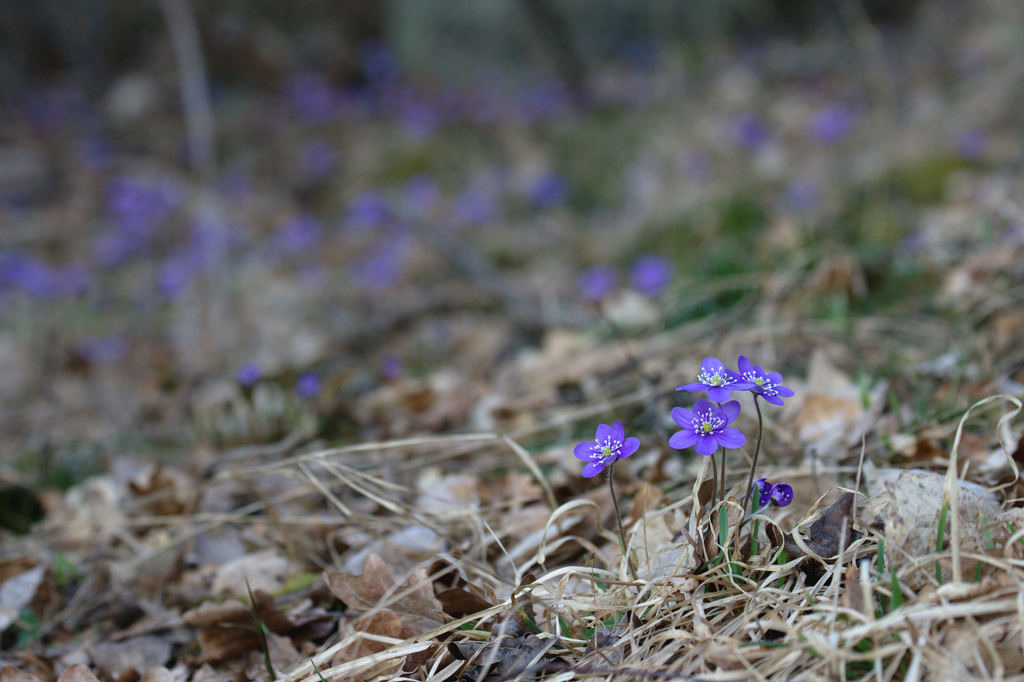
\includegraphics[height=1.5\paperheight]{Figures/blasippa.jpg}
        }   
        \parbox[c][\paperheight]{\paperwidth}{%
            \vskip 25 ex \hskip -40 em
            \color{white}\fbox{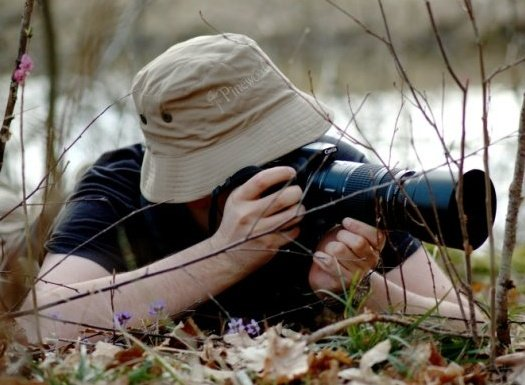
\includegraphics[height=0.37\paperheight]{Figures/me.jpg}}
        }   
    }
    \begin{frame}[plain]
        \vfill\hfill{\Huge\qquad\color{white} \zB Thank \zC you}\hfill\hfill\hfill\vfill
    \end{frame}
    \setbeamertemplate{background}{}

\end{document}
